\documentclass[
  bibliography=totoc,     % Literatur im Inhaltsverzeichnis
  captions=tableheading,  % Tabellenüberschriften
  titlepage=firstiscover, % Titelseite ist Deckblatt
]{scrartcl}

% Paket float verbessern
\usepackage{scrhack}

% Warnung, falls nochmal kompiliert werden muss
\usepackage[aux]{rerunfilecheck}

% unverzichtbare Mathe-Befehle
\usepackage{amsmath}
% viele Mathe-Symbole
\usepackage{amssymb}
% Erweiterungen für amsmath
\usepackage{mathtools}

% Fonteinstellungen
\usepackage{fontspec}
% Latin Modern Fonts werden automatisch geladen
% Alternativ zum Beispiel:
%\setromanfont{Libertinus Serif}
%\setsansfont{Libertinus Sans}
%\setmonofont{Libertinus Mono}

% Wenn man andere Schriftarten gesetzt hat,
% sollte man das Seiten-Layout neu berechnen lassen
\recalctypearea{}

% deutsche Spracheinstellungen
\usepackage[ngerman]{babel}

\usepackage[table]{xcolor}

\usepackage[
  math-style=ISO,    % ┐
  bold-style=ISO,    % │
  sans-style=italic, % │ ISO-Standard folgen
  nabla=upright,     % │
  partial=upright,   % ┘
  warnings-off={           % ┐
    mathtools-colon,       % │ unnötige Warnungen ausschalten
    mathtools-overbracket, % │
  },                       % ┘
]{unicode-math}

% traditionelle Fonts für Mathematik
\setmathfont{Latin Modern Math}
% Alternativ zum Beispiel:
%\setmathfont{Libertinus Math}

\setmathfont{XITS Math}[range={scr, bfscr}]
\setmathfont{XITS Math}[range={cal, bfcal}, StylisticSet=1]

% Zahlen und Einheiten
\usepackage[
  locale=DE,                   % deutsche Einstellungen
  separate-uncertainty=true,   % immer Unsicherheit mit \pm
  per-mode=symbol-or-fraction, % / in inline math, fraction in display math
]{siunitx}

% chemische Formeln
\usepackage[
  version=4,
  math-greek=default, % ┐ mit unicode-math zusammenarbeiten
  text-greek=default, % ┘
]{mhchem}

% richtige Anführungszeichen
\usepackage[autostyle]{csquotes}

% schöne Brüche im Text
\usepackage{xfrac}

% Standardplatzierung für Floats einstellen
\usepackage{float}
\floatplacement{figure}{htbp}
\floatplacement{table}{htbp}

% Floats innerhalb einer Section halten
\usepackage[
  section, % Floats innerhalb der Section halten
  below,   % unterhalb der Section aber auf der selben Seite ist ok
]{placeins}

% Seite drehen für breite Tabellen: landscape Umgebung
\usepackage{pdflscape}

% Captions schöner machen.
\usepackage[
  labelfont=bf,        % Tabelle x: Abbildung y: ist jetzt fett
  font=small,          % Schrift etwas kleiner als Dokument
  width=0.9\textwidth, % maximale Breite einer Caption schmaler
]{caption}
% subfigure, subtable, subref
\usepackage{subcaption}

% Grafiken können eingebunden werden
\usepackage{graphicx}

% schöne Tabellen
\usepackage{booktabs}

% Verbesserungen am Schriftbild
\usepackage{microtype}

% Literaturverzeichnis
\usepackage[
  backend=biber,
]{biblatex}
% Quellendatenbank
\addbibresource{lit.bib}
%\addbibresource{programme.bib}
%\bibliographystyle{plain}
%\bibliography{lit.bib}

% Hyperlinks im Dokument
\usepackage[
  german,
  unicode,        % Unicode in PDF-Attributen erlauben
  pdfusetitle,    % Titel, Autoren und Datum als PDF-Attribute
  pdfcreator={},  % ┐ PDF-Attribute säubern
  pdfproducer={}, % ┘
]{hyperref}
% erweiterte Bookmarks im PDF
\usepackage{bookmark}

% Trennung von Wörtern mit Strichen
\usepackage[shortcuts]{extdash}

\author{%
  AUTOR A\\%
  \href{mailto:authorA@udo.edu}{authorA@udo.edu}%
  \and%
  AUTOR B\\%
  \href{mailto:authorB@udo.edu}{authorB@udo.edu}%
}
\publishers{TU Dortmund – Fakultät Physik}


\subject{V703}
\title{Das Geiger-Müller-Zählrohr}
\author{Umut Aydinli \\
 \href{mailto:umut.aydinli@tu-dortmund.de}{umut.aydinli@tu-dortmund.de}
 \and Muhammed-Sinan Demir \\
 \href{mailto:sinan.demir@tu-dortmund.de}{sinan.demir@tu-dortmund.de}
 }
\date{
  Durchführung: 07.06.2022
  \hspace{3em}
  Abgabe: 14.06.2022
}


\begin{document}

\maketitle
\tableofcontents
\newpage

\section{Zielsetzung} 

\begin{flushleft}
    In dem Versuch V602 geht es um die Bestimmung des Emissionsspektrums einer Kupferröntgenröhre, das Absorptionsspektrum verschiedener Stoffe und die Überprüfung der Bragg Bedingung. 
\end{flushleft}



\section{Theorie}


\begin{flushleft}
    Licht besteht aus elektromagnetischen Wellen und ist somit durch die Maxwell Gleichungen beschreibbar.
    Licht, welches im sichtbaren Bereich liegt, hat eine Wellenlänge zwischen $380\unit{\nano\meter}$ und $780\unit{\nano\meter}$.
    Das Ultraviolette Spektrum liegt unter den $380\unit{\nano\meter}$ bzw. zwischen $100\unit{\nano\meter}$ und $380\unit{\nano\meter}$, wobei das Infrarotspektrum über den $780\unit{\nano\meter}$ liegt, genauer gesagt zwischen $780\unit{\nano\meter}$ und $1\unit{\milli\meter}$
\end{flushleft}

\subsection{Strahlenoptik}

\begin{align}
    \intertext{Die Wellennormale beschreibt in der Strahlenoptik die Ausbreitung der Welle.
    Dabei ist die Ausbreitungsgeschwindigkeit unterschiedlich groß, welches von dem Material abhängt.
    Beim Auftreffen eines Lichtstrahles auf die Grenzfläche eines Mediums wird der Lichtstrahl gebrochen.
    Dabei entstehen zwei Ausbreitungsgeschwindigkeiten, $\text{v}_{1}$ und $\text{v}_{2}$, die durch die beiden Brechungsindizes der Medien, $\text{n}_{1}$ und $\text{n}_{2}$, sowie durch den Einfallswinkel $\alpha$ und Brechungswinkel $\beta$ beschrieben werden können  }
    \frac{\sin(\alpha)}{\sin(\beta)} = \frac{\text{v}_{1}}{\text{v}_{2}} = \frac{\text{n}_{2}}{\text{n}_{1}}\,. \label{1}
    \intertext{Luft ist ebenfalls ein Medium, dessen Ausbreitungsgeschwindigkeit bei $ \text{v}_{1} = 2,9979 \cdot 10^{8} \frac{\unit{\meter}}{\unit{\second}} $ liegt und einen Brechungsindex von $\text{n}_{1} = 1,000292$ besitzt.
    Das Medium,in welchen die Ausbreitungsgeschwindigkeit des Lichts größer ist als in dem anderen Medium, gilt als optisch dichteres Medium.
    Dadurch gilt, dass bei geringerer Ausbreitungsgeschwindigkeit von einem optisch dünneren Medium gesprochen wird.  }
\end{align}

\subsection{Reflexion} 

\begin{align}
    \intertext{Das Reflexionsgesetz besagt, dass wenn ein Lichtstrahl auf eine Grenzfläche auftrifft und reflektiert wird, ist der Einfallswinkel gleich dem Ausfallswinkel }
    \alpha_{1} = \alpha_{2}\,. \label{2}
\end{align}

\begin{figure}[H]
    \centering
    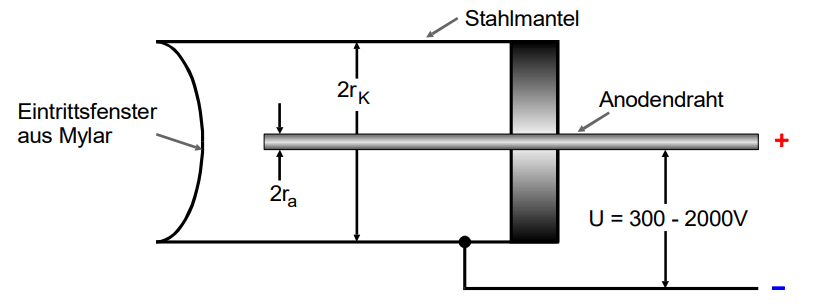
\includegraphics[height=40mm]{bilder/Ab1.png}
    \caption{Das reflektieren eines Lichtstrahles \cite{a1}.\label{Abbildung1} }
\end{figure}


\subsection{Brechung} 

\begin{align}
    \intertext{Brechung des Lichtes wird mit dem Snellius Gesetz erklärt, welches besagt, dass beim Auftreffen eines Lichtstrahl auf ein anderes Medium mit einem Brechungsindex n, dieser gebrochen wird.
    Dadurch wird der Ausfallswinkel als $\beta$ beschrieben}
    \text{n}_{1} \sin(\alpha) = \text{n}_{2} \sin(\beta)\,.\label{3}
\end{align}

\begin{figure}[H]
    \centering
    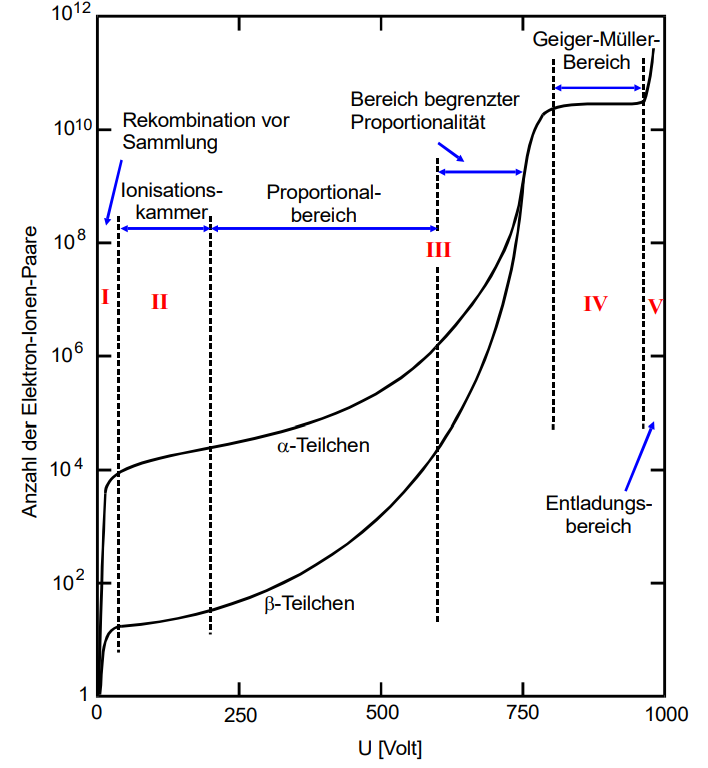
\includegraphics[height=45mm]{bilder/Ab2.png}
    \caption{Das brechen eines Lichtstrahles \cite{a1}. \label{Abbildung2} }
\end{figure}

\subsection{Reflexion und Transmission}

\begin{align}
    \intertext{Oft wird Licht nicht vollständig reflektiert, wenn es auf die Grenzfläche eines Mediums trifft.
    Der Teil des Lichtstrahles, der nicht reflektiert wird, wird transmittiert bzw. gebrochen.
    Dabei gilt das der Teil der reflektiert wird und der Teil der gebrochen wird, zusammen 1 ergibt}
    \text{R} + \text{T} = 1\,. \notag
\end{align}

\begin{figure}[H]
    \centering
    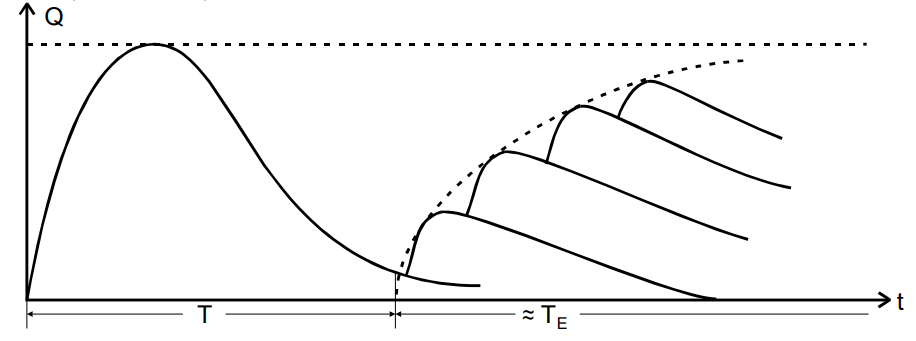
\includegraphics[height=45mm]{bilder/Ab3.png}
    \caption{Das reflektieren und brechen eines Lichtstrahles \cite{a1}. \label{Abbildung3} }
\end{figure}

\subsection{Wellenoptik}

\begin{flushleft}
    Beim Auftreffen des Lichtes auf ein Objekt, welches im Verhältnis zur Wellenlänge klein ist, breitet sich dieses auch im Schattenraum aus, da die geometrische Optik dafür nicht mehr ausreicht.
    Dabei sind Frequenz f, Wellenlänge $\lambda$ und Ausbreitungsgeschwindigkeit v, charakteristische Merkmale einer Welle, dessen Wellenzüge nicht länger als $10^{-8}\,\unit{\second}$ dauern.
    Durch eine Superpostion der Wellen können dennoch Interferenzbilder entstehen, wobei unter konstruktiver und destruktiver Interferenz unterschieden wird. 
    Beträgt der Gangunterschied bei gleicher Intensität $\lambda/2$, führt dies zu einer vollständigen Auslöschung der Welle.
\end{flushleft}

\subsection{Beugung am Gitter}

\begin{align}
    \intertext{Liegt bei der Ausbreiten der Lichtwelle ein Hindernis auf dem Weg, welches im Vergleich zur Wellenlänge klein ist, so kann es zu einer Beugung führen.
    Das Huygensche Prinzip beschreibt diese Ausbreitung und besagt, dass jeder Punkt auf einer Wellenfront eine neue Elementarwelle, welche die gleiche Frequenz hat, erzeugt.
    Befindet sich nun ein Spalt im Abstand L mit einem Schirm dahinter, wird ein Interferenzmuster beobachtbar. 
    Die dabei entstehenden Interferenzmaxima ergeben sich durch   }
    \text{a}\,\,\sin(\alpha) = \text{k}\,\lambda \,, \label{4}
    \intertext{wobei a die Spaltbreite, k das k-te Intensitätsminimum und $\lambda$ die Wellenlänge darstellt.
    Diese Intensitätsminima befindet sich in einem Winkel von $\alpha$ relativ zur geradlinigen Ausbreitungsrichtung.
    Dieses Prinzip lässt sich auf ein Strichgitter mit n-Einfachspalten gleicher Breite, mit der Gitterkonstante d, übernehmen.
    Dadurch ergibt sich für die Interferenzmaxima k-ter Ordnung die Beziehung }
    \text{d}\,\,\sin(\alpha) = \text{k}\,\lambda\,. \label{5}
\end{align}
\section{Versuchsaufbau und Versuchsdurchführung}

\begin{flushleft}
    Der Aufbau für diesen Versuch besteht aus einer Kupfer-Röntgenröhre, einem KBr-Kristall, einem Geiger-Müller-Zählrohr und einem Rechner mit dem Programm measure.
    Die Röntgenröhre kann manuell aber auch mit dem Rechner bedient werden, jedoch werden in diesem Versuch alle Messungen mit dem Rechner aufgenommen.
    In dem Programm werden folgende Einstellungen gewählt: \\
    In der oberen Zeile des Programms wird unter dem Menüpunkt Messgerät, Röntgengerät ausgewählt. 
    Unter Messart können Drehmodus, Kristallwinkel, Spektren, Beschleunigungsspannung, Emissionsstrom, Startwinkel sowie Stopwinkel und die Integrationszeit eingestellt werden und die Messung nach einstellen starten.
    Der Emissionsstrom wird dabei durchgehend auf $1\,\unit{\milli\ampere}$ und die Beschleunigungsspannung auf $35\,\unit{\kilo\volt}$ gestellt. 
\end{flushleft}

\begin{figure}[H]
    \centering
    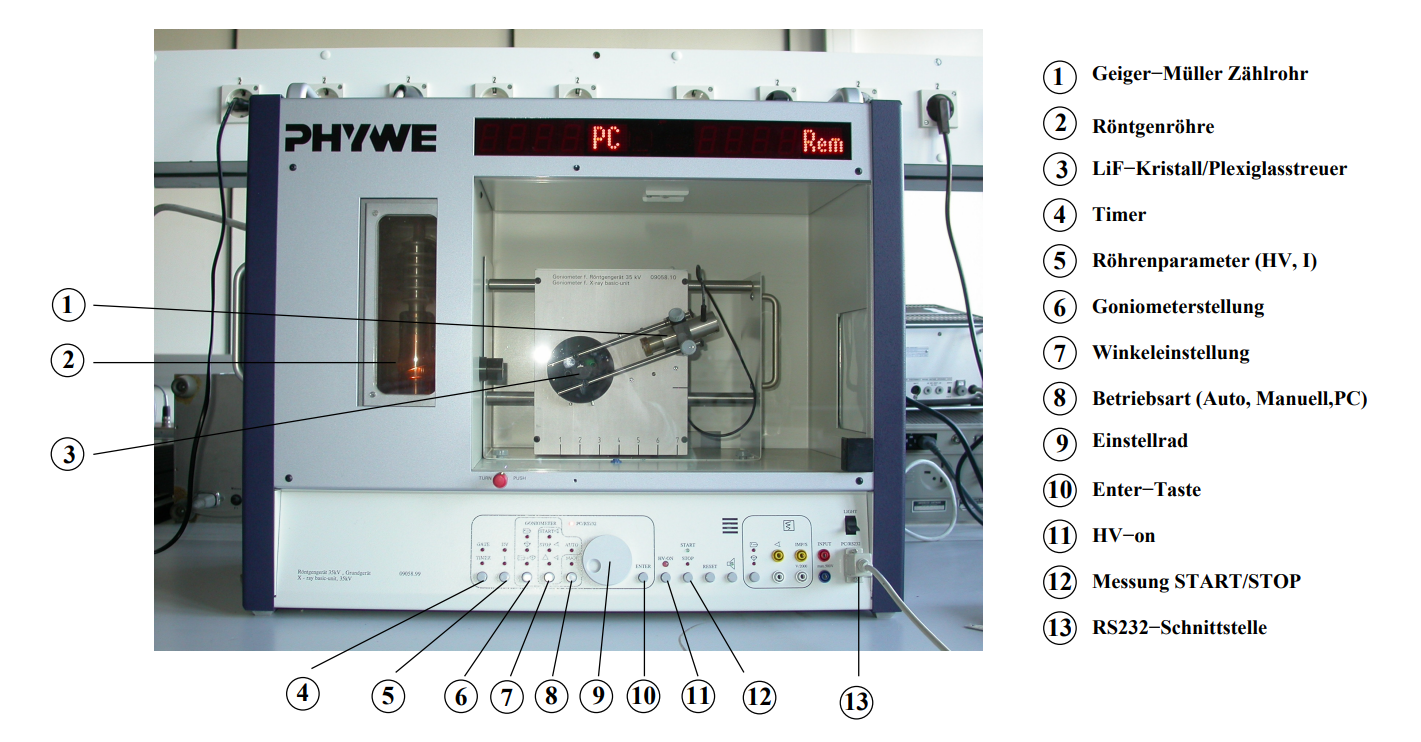
\includegraphics[height=80mm]{bilder/Röntgenröhre.png}
    \caption{Röntgenröhre mit Geiger-Müller-Zählrohr \cite{a1}. \label{Abbildung2} }
\end{figure}

\subsection{Überprüfung der Bragg Bedingung}

\begin{flushleft}
    Um die Bragg Bedingung zu überprüfen wird in dem Programm der Kristall auf einen Festwinkel von $\theta = 14\unit{\degree}$ eingestellt. 
    Der Startwinkel wird auf $\alpha_{\text{Gm}} = 26\unit{\degree}$, der Stopwinkel wird auf $\alpha_{\text{Gm}} = 30\unit{\degree}$, der Winkelzuwachs wird auf $\increment \alpha = 0,1\unit{\degree}$ und die Integrationszeit wird auf $\increment \text{t} = 5\,\unit{\second}$ gestellt.
    Danach kann die Messung gestartet und mit den gemessenen Daten das Maximum der Kurve bestimmt werden.
    Diese wird dann mit dem Sollwinkel verglichen und bei mehr als $1\unit{\degree}$ Unterschied muss der Assistent oder die Praktikumsleitung informiert werden.
\end{flushleft}

\subsection{Das Emissionsspektrum einer Cu-Röntgenröhre}

\begin{flushleft}
    Um das Emissionsspektrum der Kupferröhre zu bestimmen wird unter dem Menüpunkt Messart der 2:1 Koppelmodus ausgewählt, der Startwinkel auf $\alpha = 4\unit{\degree}$ und der Stopwinkel auf $\theta = 26\unit{\degree}$ gesetzt.
    Der Winkelzuwachs wird auf $0,2\unit{\degree}$ und die Integrationszeit auf $\increment t = 5\,\unit{\second}$ gesetzt.
    Danach kann die Messung gestartet werden.
\end{flushleft}

\subsection{Das Absorptionsspektrum}

\begin{flushleft}
    Für die Bestimmung des Absorptionsspektrums der fünf verschiedenen Stoffe, welche in der Vorbereitungsaufgabe vorkamen, wird die Integrationszeit auf $\increment t = 20\,\unit{\second}$ und der Winkelzuwachs auf $0,1\unit{\degree}$ gesetzt.
    Die jeweiligen Proben werden an dem Geiger-Müller-Zählrohr, mit Festziehen der an der Probe vorhandenen Schraube, befestigt.
    Start und Stopwinkel werden individuell über den in der Vorbereitungsaufgabe berechneten Winkel angepasst.
    Es sollten jedoch ca. $\pm\, 1\unit{\degree}\,\, \text{bis} \,\, 2\unit{\degree}$ der berechneten Winkels als Start- Stopwinkel gewählt werden.
    Dies wird für alle fünf Stoffe wiederholt.
\end{flushleft}
\section{Auswertung}

\subsection{Messunsicherheiten}

\begin{align*}
    \intertext{Bei fehlerhafteten Größen wird der neue Fehler mithilfe von Gauß´schen Fehlerfortpflanzung angegeben}\\
    \increment f = \sqrt{\frac{N}{i=1} \cdot (\frac{\partial f}{\partial x_{i}}^2) \cdot (\increment x_{i}) }.
\end{align*} 

\subsection{Auswertung des erstens Durchlaufs}

\begin{flushleft}
    Die Konstruktion besteht aus zwei Pendel, die nicht mit einer Feder verbunden worden sind. 
    Die Länge der beiden Pendel beträgt $ l_{1,2} = 0,78 \, \unit{\meter} $.
    Die Massen haben je ein Gewicht von $ m_{1,2} = 1\, \unit{\kilo\gram} $.
    Beide Pendel werden jeweils um $ \increment x_{Auslenkung} = 0,075 \, \unit{\meter} $ ausgelenkt. 
    Die gemessene Schwingungsdauer besteht aus fünf Schwingungen.
\end{flushleft} 

\begin{table}[H]
    \centering
    \caption{Die Messwerte der freischwingenden Pendel des ersten Durchgangs.}
    \label{Tabelle1}
    \begin{tabular} {c  c}
        \toprule
        {$T_{1,v1} \mathbin{/} \unit{\second}$} &
        {$T_{2,v1} \mathbin{/} \unit{\second}$} \\
        \midrule
         8,83 & 8,91 \\
         8,75 & 8,86 \\
         8,86 & 8,63 \\
         8,83 & 8,65\\
         8,78 & 8,62 \\
         8,93 & 8,51 \\
         8,82 & 8,53 \\
         8,53 & 8,88 \\
         8,72 & 8,61 \\ 
         8,67 & 8,81 \\
        \bottomrule
    \end{tabular} 
\end{table}

\begin{align*}
    \intertext{Die Werte werden gemittelt und die dazugehörige Standardabweichung bestimmt, sowie auf eine Periodenschwingung normiert }\\
    T_{1,Pendel 1} = (1,754 \pm 0,025)\, \unit{\second}\\
    T_{2,Pendel 2} = (1,740 \pm 0,029)\, \unit{\second}.
\end{align*}

\underline{\textbf{Experimentelle Bestimmung}}

\begin{flushleft}
    Die Pendel behalten ihre Länge und werden erneut um $ 0,075\, \unit{\meter} $ ausgelenkt.
\end{flushleft}

\begin{table}[H]
    \centering
    \caption{Die Messwerte der gleichphasigen Schwingung des ersten Durchgangs.}
    \label{Tabelle2}
    \begin{tabular} {c}
        \toprule
        {$ T_{+,v1 } \mathbin{/} \unit{\second} $} \\
        \midrule
         8,54 \\
         8,59 \\
         8,74 \\
         8,47 \\
         8,77 \\
         8,54 \\
         8,75 \\
         8,37 \\
         8,72 \\
         8,43 \\
         8,57 \\
        \bottomrule
    \end{tabular} 
\end{table}

\begin{align*}
    \intertext{Für die Schwingungsdauer $T_{+}$ folgt}\\
    T_{+,v1} = (1,718 \pm 0,027)\, \unit{\second}.\\
    \intertext{Die Frequenz hat nach der Formel (\ref{1}), einen Wert von}\\
    \omega_{+,exp,v1} = (3,657 \pm 0,0117)\, \frac{1}{s}.
\end{align*}

\begin{flushleft}
    Für die gegenphasige Schwingung werden beide Pendel nach innen um $ 0,055\, \unit{\meter} $ ausgelenkt.
\end{flushleft}

\begin{table}[H] 
    \centering
    \caption{Die Messwerte der gegenphasigen Schwingung des ersten Durchgangs.}
    \label{Tabelle3}
    \begin{tabular} {c}
        \toprule
        {$ T_{-,v1 } \mathbin{/} \unit{\second} $} \\
        \midrule
         8,34 \\
         8,09 \\
         8,17 \\
         7.99 \\
         8,22 \\
         8,14 \\
         8,10 \\
         8,20 \\
         8,02 \\
         8,11 \\
        \bottomrule
    \end{tabular} 
\end{table}

\begin{align*}
    \intertext{Für die Schwingungsdauer $ T_{-} $ folgt} \\
    T_{-,v1} = (1,629 \pm 0,02)\, \unit{\second}.\\
    \intertext{Die Frequenz lässt sich ableiten durch die Formel (\ref{3})}\\
    \omega_{-,exp,v1} = (3,855 \pm 0,0097)\, \frac{1}{s}. \\
    \intertext{Die Kopplungskonstante errechnet sich durch die Formel (\ref{7}). } \\
    \intertext{Es ergibt sich}\\
    K_{v1} = (0,0527 \pm 0,1347).
\end{align*}

\underline{\textbf{Theoretische Bestimmung}}

\begin{flushleft}
    Die Frequenz bestimmt sich durch die Formel (\ref{1}) unter der Beachtung, dass fünf Schwingungen gemessen worden sind.
\end{flushleft}

\begin{align*}
    \intertext{Für die Gleichphasige Schwingung ergibt sich}\\
    \omega_{+,theo,v1} = (3,546 \pm 0,0228 )\, \frac{1}{s}.\\
    \intertext{Daraus, aus der Formel (\ref{2}), die Dauer }\\
    T_{+,theo,v1} = (1,771 \pm 0,002 )\, \unit{\second}.\\
    \intertext{Die Gegenphasige wird mit den Formeln (\ref{3}) und (\ref{4}) bestimmt, dabei wird die Kopplungskonstante $K$ aus der experimentellen Herleitung genommen. Unter der Beachtung der Fehler}\\  
    \omega_{-,theo,v1} = ( 3,5653 \pm 0,0504 )\, \frac{1}{s} \\
    T_{-,theo,v1} = (1,762 \pm 0,004 )\, \unit{\second}. \\
\end{align*}


\begin{flushleft}
    Um die Schwebungsdauer zu bestimmen, wird ein Pendel, $Pendel_{1}$, in die Ruhelage versetzt und $ Pendel_{2} $ um 
    $ \alpha_{2} \neq 0 $ ausgelenkt, in unserem Fall $ \increment x_{schw,Ausl} = 0,075\, \unit{\meter} $.
    Die Pendellänge bleibt erhalten.
\end{flushleft}

\begin{table}[H]
    \centering
    \caption{Die Messwerte der gekoppelten Schwingung des ersten Durchgangs.}
    \label{Tabelle4}
    \begin{tabular} {c  c}
        \toprule
        {$ T_{Gs,v1} \mathbin{/} \unit{\second}$} &
        {$ T_{Schw.,v1} \mathbin{/} \unit{\second}$} \\
        \midrule
         9,22 & 19,68 \\
         8,80 & 19,46 \\
         9,10 & 19,51 \\
         8,55 & 19,10 \\
         8,99 & 18,91 \\
         8,67 & 19,45 \\
         8,64 & 19,34 \\
         8,52 & 19,92 \\
         8,65 & 18,76 \\
         8,73 & 19,15 \\
        \bottomrule
    \end{tabular} 
\end{table}

\begin{align*}
    \intertext{Die Werte werden gemittelt und die Abweichung bestimmt}\\
    T_{Gs,v1} = (1,757 \pm 0,047)\, \unit{\second}\\
    T_{Schw.,v1} = (19,328 \pm 0,3529 )\, \unit{\second}.\\
    \intertext{Für die Schwebungsfrequenz ergibt sich aus dem Kehrwert der Schwebungsdauer}
    \omega_{s,exp} = ( 0,0517 \pm 0,0009 )\, \frac{1}{s}. \\ 
    \intertext{Die Schwingungsdauer wird mithilfe der gleichphasigen und gegensinnigen Schwingung berechnet mit der Formel (\ref{5}):}\\
    T_{S} = (22,57 \pm 0,6110 )\, \unit{\second}
    \intertext{sowie die Schwebungsfrequenz $ \omega_{s} $ mit Formel (\ref{6}): }\\
    \left\lvert \omega_{s,theo} \right\rvert = (0,0193 \pm 0,0151 )\, \frac{1}{s}.
\end{align*}

\subsection{Auswertung für den zweiten Durchlauf}

\underline{\textbf{Experimentelle Bestimmung}}

\begin{flushleft}
    Die Konstruktion bleibt erhalten. Man geht vor wie im ersten Durchgang vor, nur hierbei wurde die Pendellänge auf $ l = 0,99\, \unit{\meter} $
    erweitert.
\end{flushleft}

\begin{table}[H]
    \centering
    \caption{Die Messwerte der frei schwingenden Pendel des zweiten Durchgangs.}
    \label{Tabelle5}
    \begin{tabular} {c  c}
        \toprule
        {$T_{1,v2} \mathbin{/} \unit{\second}$} &
        {$T_{2,v2} \mathbin{/} \unit{\second}$} \\
        \midrule
         9,67 & 9,75 \\
         9,87 & 9,63 \\
         9,86 & 9,82 \\
         9,73 & 9,73\\
         9,87 & 9,63 \\
         9,79 & 9,69 \\
         9,58 & 9,41 \\
         9,53 & 9,69 \\
         9,72 & 9,74 \\ 
         9,72 & 9,73 \\
        \bottomrule
    \end{tabular} 
\end{table} 

\begin{align*} 
    \intertext{Daraus folgt experimentell}\\
    T_{1,exp,v2} = (1,946 \pm 0,0236 )\, \unit{\second} \\
    T_{2,exp,v2} = (1,936 \pm 0,0222 )\, \unit{\second}.
\end{align*}


\begin{table}[H]
    \centering
    \caption{Die Messwerte der gleichphasigen und gegenphasigen Schwingung des zweiten Durchgangs.}
    \label{Tabelle6}
    \begin{tabular} {c  c}
        \toprule
        {$ T_{gl,v2 } \mathbin{/} \unit{\second} $} &
        {$ T_{gg,v2} \mathbin{/} \unit{\second} $} \\
        \midrule
        9,62 & 9,47 \\
        9,60 & 9,22 \\
        9,67 & 9,20 \\
        9,44 & 9,08 \\
        9,32 & 9,05 \\
        9,74 & 9,13 \\
        9,77 & 9,93 \\
        9,69 & 9,27 \\
        9,45 & 9,25 \\
        9,67 & 9,27 \\
        \bottomrule
    \end{tabular} 
\end{table} 

\begin{align*}
    \intertext{Daraus folgt:}\\
    T_{+,exp,v2} = (1,919 \pm 0,029 )\, \unit{\second} \\
    T_{-,exp,v2} = (1,857 \pm 0,050 )\, \unit{\second}. \\
    \intertext{Mit der Kreisfrequenz aus den Formeln (\ref{1}) und (\ref{3})}\\
    \omega_{+,exp,v2} = (3,27 \pm 0,009 )\, \frac{1}{s}\\
    \omega_{-,exp,v2} = (3,382 \pm 0,0185 )\, \frac{1}{s}\\
    \intertext{Die Kopplungskonstante hat dabei einen Wert von}\\
    K_{v2} = ( 0,0328\pm 0,0050 )
\end{align*}


\underline{\textbf{Theoretische Bestimmung}}

\begin{align*}
    \intertext{Für die Gleichphasige Schwingung ergibt sich nach der Formel (\ref{1}):}\\
    \omega_{+,theo,v2} = (3,147 \pm 0,0159 )\, \unit{\second}.\\
    \intertext{Daraus, aus der Formel (\ref{2}), die Dauer}\\
    T_{+,theo,v2} = (1,996 \pm 0,002 )\, \unit{\second}.\\
    \intertext{Für die Gegenphasige Schwingung folgt nach der Formel (\ref{3}) und (\ref{4})} \\
    \omega_{-,theo,v2} = ( 3,1583 \pm 0,0157)\, \frac{1}{s}\\
    T_{-,theo,v2} = ( 1,989\pm 0,002 )\, \unit{\second}\\
    \intertext{Für die Schwebedauer wird die selbe Einstellung gewählt, nur die Pendellänge wird auf $ 0,99\, \unit{\meter} $ gesetzt.
    Die Auswertung ist wie im ersten Durchgang.}
\end{align*}

\begin{table}[H]
    \centering
    \caption{Die Messwerte der gekoppelten Schwingung des zweiten Durchgangs.}
    \label{Tabelle7}
    \begin{tabular} {c  c}
        \toprule
        {$ T_{gs,v2} \mathbin{/} \unit{\second}$} &
        {$ T_{s} \mathbin{/} \unit{\second}$} \\
        \midrule
         11,13 & 26,24 \\
         12,41 & 26,94 \\
         10,93 & 25,44 \\
         11,58 & 25,90 \\
         11,25 & 26,22 \\
         11,32 & 26,51 \\
         11,65 & 25,69 \\
         11,73 & 27,07 \\
         11,38 & 26,86 \\
         11,31 & 26,78 \\
        \bottomrule
    \end{tabular} 
\end{table}

\begin{align*}
    \intertext{Daraus folgt:}\\
    T_{gs,exp,v2} = (2,293 \pm 0,081 )\, \unit{\second}\\
    T_{schw.,exp,v2} = (26,425 \pm 0,6667)\, \unit{\second}\\
    \intertext{Aus dem Kehrwert der Schwebungsdauer resultiert für die Frequenz}
    \omega_{s,exp} = (0,037 \pm 0,0004 )\, \frac{1}{s}. \\
    \intertext{Die Schwebungsdauer wird mithilfe der gleichphasigen und gegensinnigen Schwingung berechnet, mit der Formel (\ref{5}). Es ergibt sich}\\
    T_{s} = (28,70 \pm 0,2447 )\, \unit{\second}\\
    \intertext{Mit der Formel (\ref{6}) für die Schwebungsfrequenz}\\
    \left\lvert \omega_{s,theo} \right\rvert = (-0,112 \pm 0,0205 )\, \frac{1}{s}.\\
\end{align*}

\begin{align}
    \intertext{Nun gilt es, die jeweiligen Werte miteinander zu vergleichen. 
    Dafür wird die Formel (\ref{8}) verwendet:}
    \text{\underline{ relative Abweichung in \% :}} \hspace{0.5cm} \frac{x_{exp} - x_{theo} }{x_{theo}} \cdot 100. \label{8}
\end{align}

\section{Diskussion}

\begin{flushleft}
    Die Ermittlung der Schallgeschwindigkeit mit der Geräteeinstellung, des Impuls-Echo-Verfahren sowie des Durchschallungs-Verfahrens weisen folgende Abweichungen auf.
\end{flushleft}

\begin{table}[H]
    \centering
    \begin{tabular} {c | c}
        \toprule
        { } &
        {Abweichung zu $ \text{c}_{\text{acryl}} = 2730\,\frac{\unit{\meter}}{\unit{\second}} $ \cite{a1} in \%} \\
        \midrule
        $\text{c}_{\text{exp}}   = 2777,7\,\frac{\unit{\meter}}{\unit{\second}} $ & 1,74 \\
        $ \text{A}_{\text{Echo}}   = 2723\,\frac{\unit{\meter}}{\unit{\second}} $ & 0,25 \\
        $ \text{A}_{\text{Durch.}} = 2663\,\frac{\unit{\meter}}{\unit{\second}} $ & 2,45 \\
        \bottomrule
    \end{tabular} 
\end{table}

\begin{flushleft}
    Die Abweichungen sind sehr gering somit erweist sich die Bestimmung der Schallgeschwindigkeit mit dem Impuls-Echo-Verfahren am profitabelsten.
\end{flushleft}

\begin{flushleft}
    Die Dicke der Scheiben haben eine Abweichung von
\end{flushleft}

\begin{table}[H]
    \centering
    \begin{tabular} {c |  c  c}
        \toprule
        { } &
        {$ \text{Scheibe}_{\text{Lit.}}\,(\text{o.})$ in \% }  &
        {$ \text{Scheibe}_{\text{Lit.}}\,(\text{u.}) $ in \%}  \\
        \midrule
        $\text{Scheibe}\,(\text{o.}) $ & 3,8 & - \\
        $\text{Scheibe}\,(\text{u.}) $  & -  & 3,3  \\
        \bottomrule
    \end{tabular} 
\end{table}

\begin{flushleft}
    Für das Abmessung der Auge lassen sich Referenzwerk finden, die ungefähr den berechneten Abständen entsprechen.
    Dennoch weisen bei der Versuchsreihe gewisse Ungenauigkeiten bzw. Abweichungen auf.
    Die Fehlerquellen liegen zum einen bei der begrenzten Ablesemöglichkeit oder die falsche Untersuchungen an den Grafiken.
    Die Ultraschallsonden sind ebenso nicht präzise bei der Messung und können mit einer begrenzten Genauigkeit die Amplituden und Laufzeiten messen.
\end{flushleft}

\begin{flushleft}
    Nichtsdestotrotz eignet sich das Verfahren zur Untersuchung von Materialien mit verschiedenen Ultraschallmessmethoden.
\end{flushleft}
\section{Anhang}

\begin{figure}
    \center
    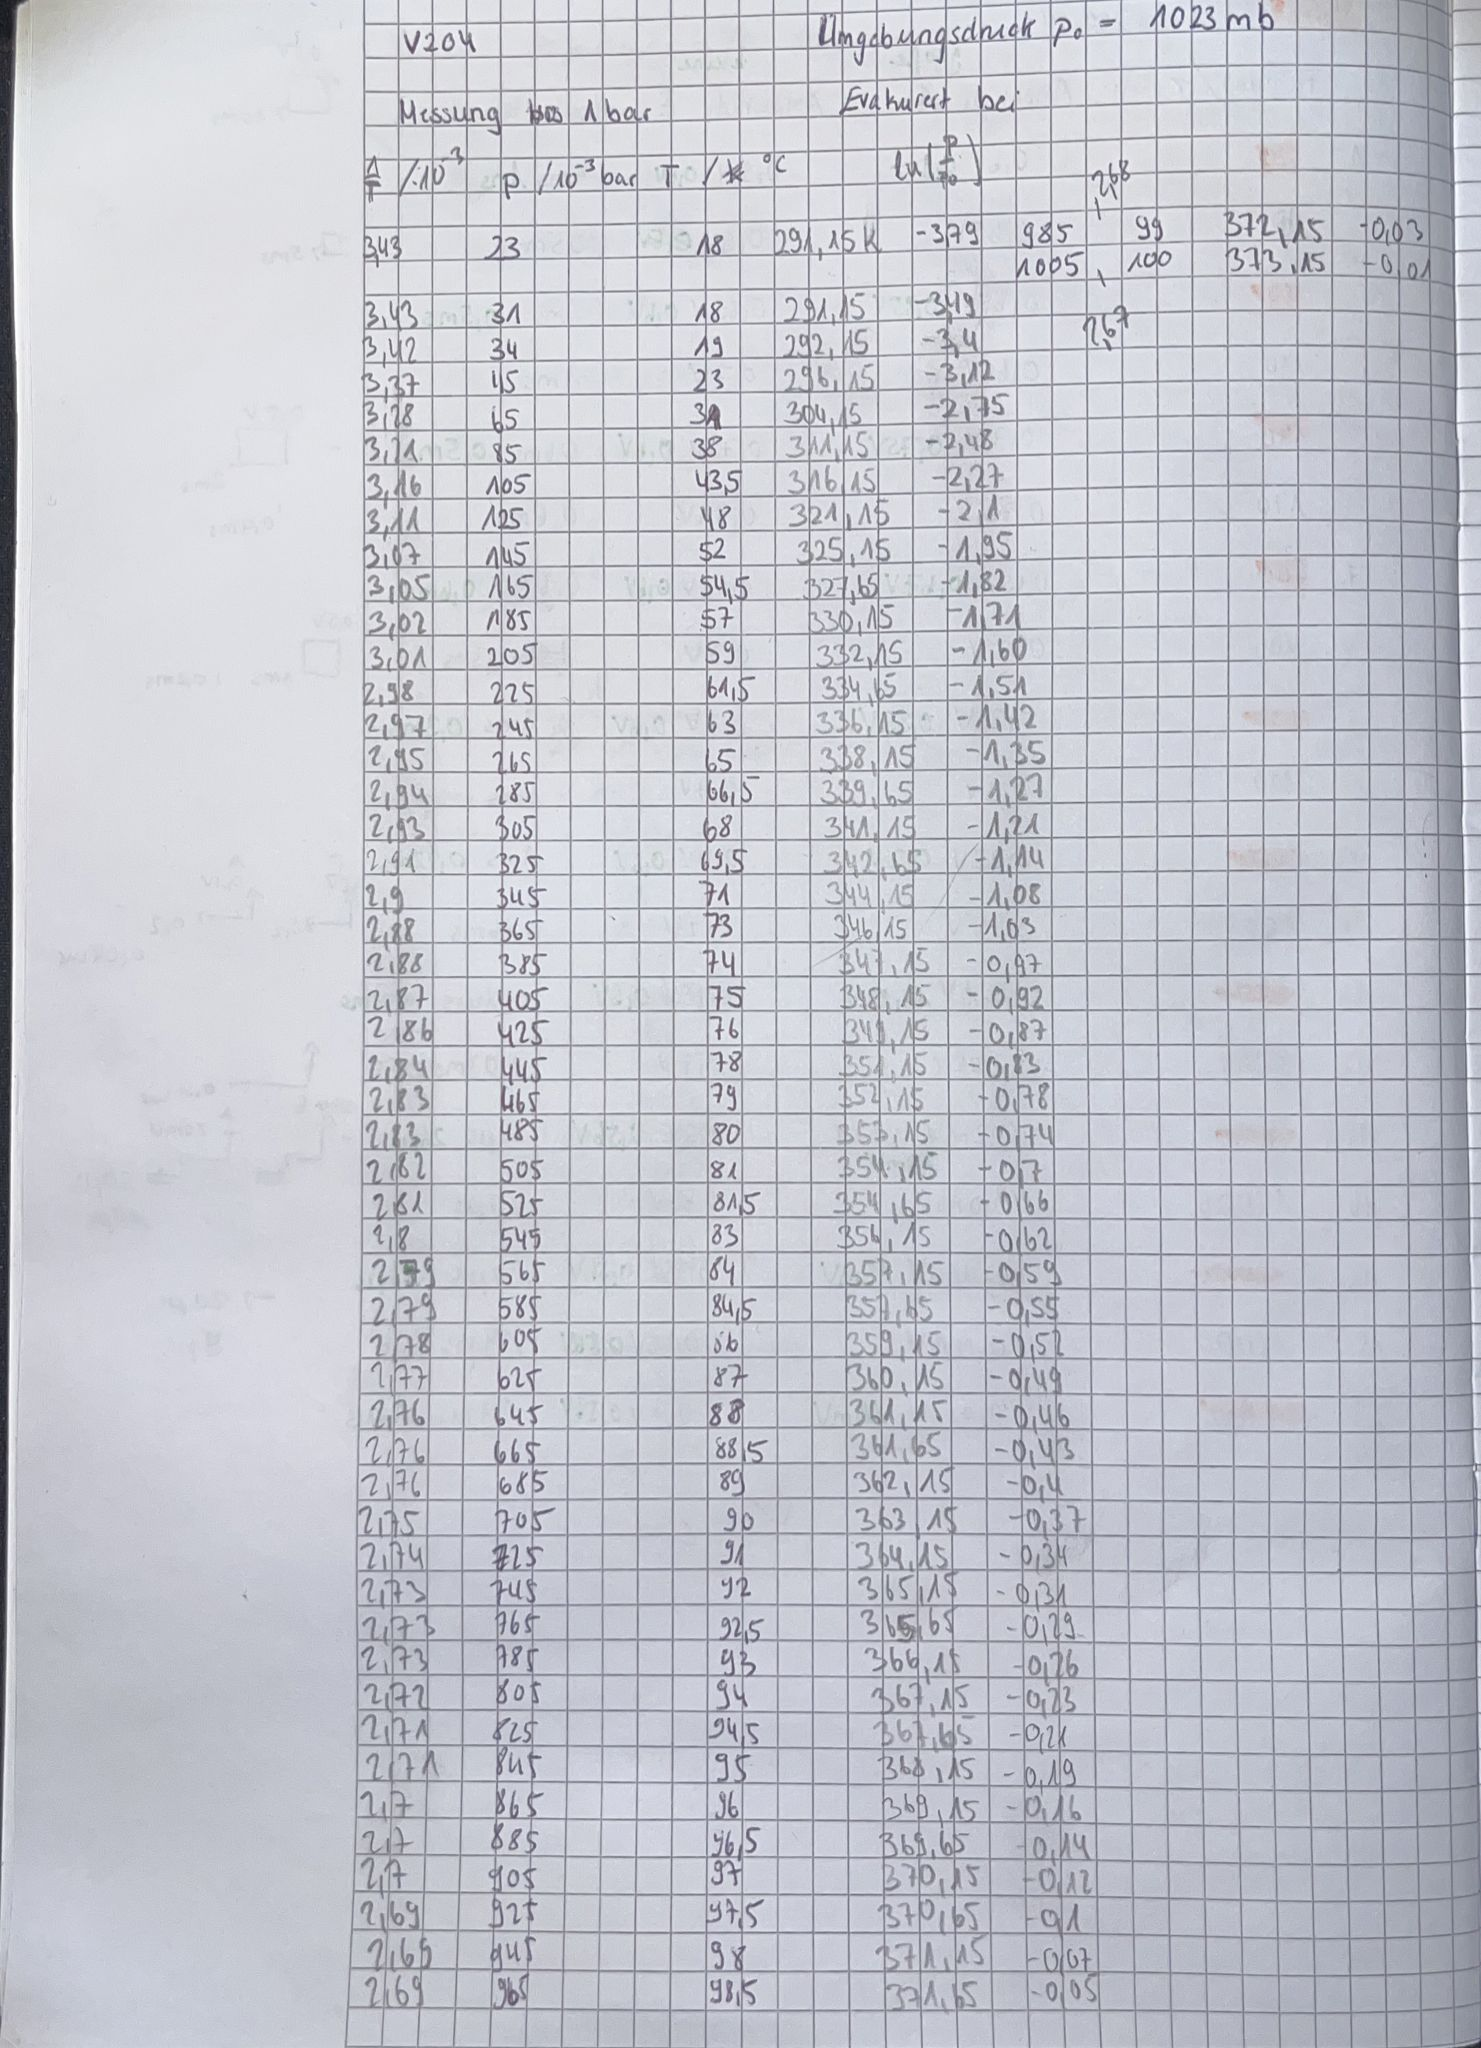
\includegraphics[width=12.5cm]{bilder/Anhang1.jpeg}
\end{figure}

\begin{figure}
    \center
    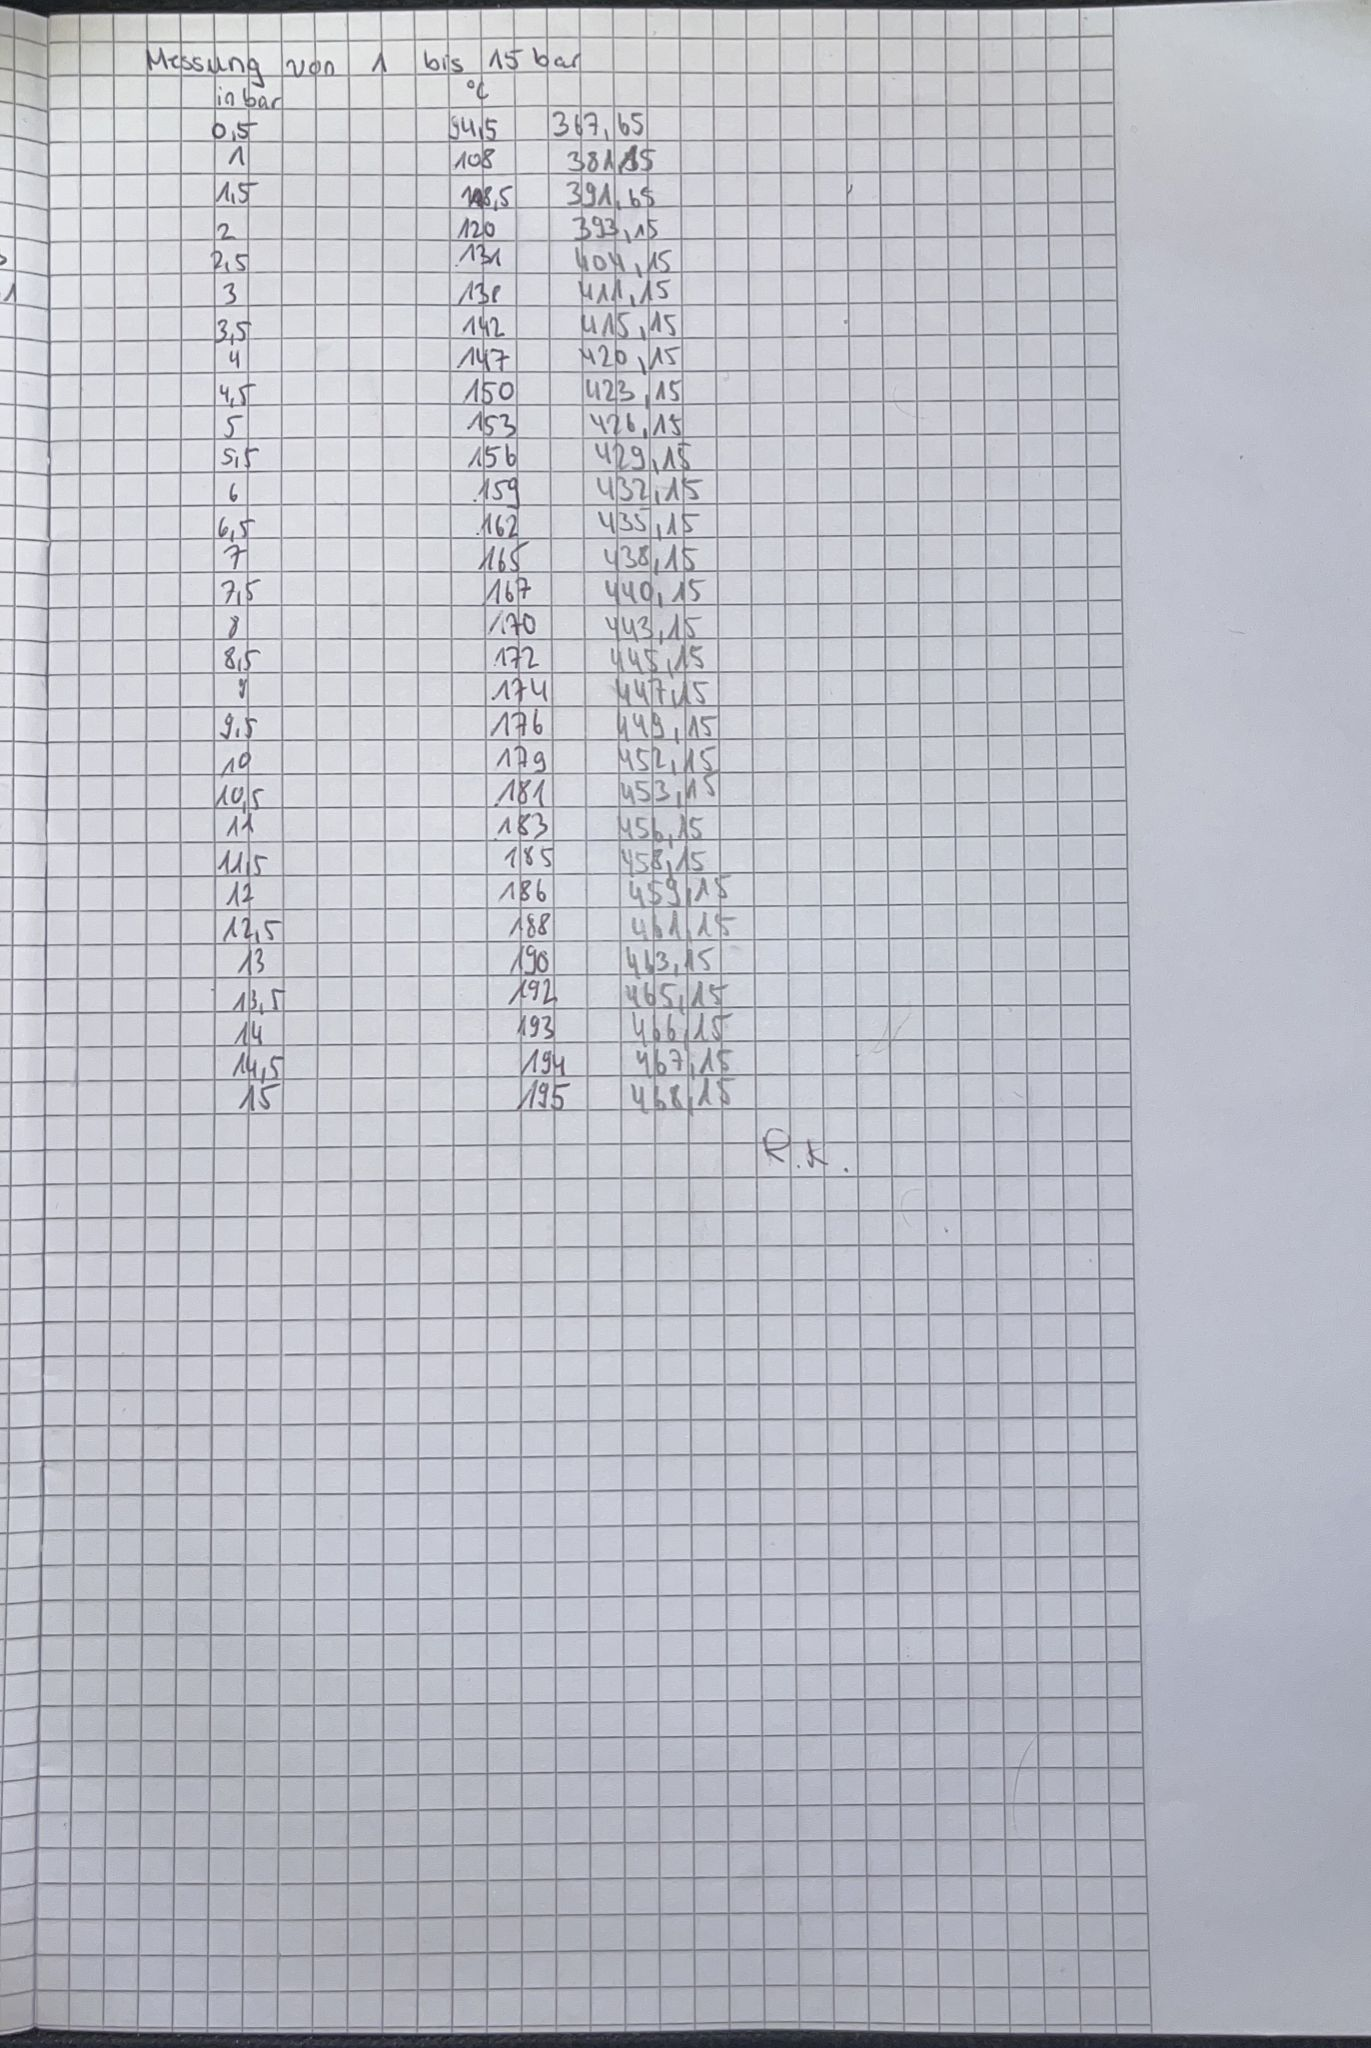
\includegraphics[width=14cm]{bilder/Anhang2.jpeg}
\end{figure}

\nocite{*}
\printbibliography{}

\end{document}